\chapter{Evaluation of Lightweight Scene Understanding}

\section{Experimental Setup}
\label{sec:segmentation-experimental-setup}

Deployment benchmarks were run on a single NVIDIA T4 GPU in the Kaggle environment. Latency was averaged over 50 forward passes after 10 warm-up runs, with synchronization ensuring that GPU execution had completed before each measurement ended. Energy and peak memory were measured in a separate loop that continued for at least 100 inference runs and 30 seconds. GPU power and memory were sampled every 20~ms through the NVIDIA Management Library (NVML), and energy per image was obtained by dividing the estimated GPU energy consumed during the loop by the number of processed images.

\section{Segmentation Accuracy}
\label{sec:segmentation-accuracy}

The various architectures were evaluated on the S5Mars test split, using the checkpoint with the highest validation mIoU for each training run. The U-Net, DeepLab, and SegFormer followed the training procedure described in Chapter~2, using 30 epochs for training, whereas the two LCNet variants were trained for 60 epochs, without data augmentation or oversampling. Table~\ref{tab:s5mars-reference-accuracy} reports the results obtained, the validation mIoU used for checkpoint selection alongside the test mIoU and pixel accuracy, keeping model selection separate from the final evaluation.

\begin{table}[ht!]
    \centering
    \small
    \setlength{\tabcolsep}{4pt}
    \begin{tabular}{@{}l c c c@{}}
        \toprule
        \textbf{Configuration}                   &
        \shortstack{\textbf{Val} \textbf{mIoU}}  &
        \shortstack{\textbf{Test} \textbf{mIoU}} & \textbf{Test PA}                 \\
        \midrule
        \midrule
        U-Net (R34)                              & 81.52            & 64.55 & 91.73 \\
        U-Net (MV2)                              & 71.98            & 64.57 & 91.22 \\
        DeepLabV3 (R34)                          & 83.14            & 73.79 & 91.63 \\
        DeepLabV3+ (MV2)                         & 80.81            & 64.07 & 90.59 \\
        SegFormer-B0                             & 80.28            & 75.55 & 91.27 \\
        \midrule
        LCNet\(_{3,7}\)                          & 60.59            & 57.89 & 88.87 \\
        LCNet\(_{3,11}\)                         & 64.54            & 59.11 & 88.98 \\
        \bottomrule
    \end{tabular}
    \vspace{5mm}
    \caption{S5Mars accuracy of the evaluated FP32 configurations. R34 and MV2 denote ResNet34 and MobileNetV2, respectively. Validation mIoU identifies the selected checkpoint, while test metrics describe its held-out performance.}
    \label{tab:s5mars-reference-accuracy}
\end{table}
SegFormer-B0 achieved the highest test mIoU, 75.55\%, followed by DeepLabV3 with ResNet34 at 73.79\%. Its accuracy is particularly relevant to the lightweight objective: with 3.72 million parameters, compared with 26.01 million for DeepLabV3, SegFormer-B0 obtained a higher mIoU with approximately 86\% fewer parameters (Table~\ref{tab:segmentation-architecture-static-comparison}). U-Net with ResNet34 achieved the highest pixel accuracy, 91.73\%, whereas SegFormer-B0 led on average IoU.

U-Net with MobileNetV2 retained essentially the same test mIoU as its ResNet34 counterpart, 64.57\% versus 64.55\%, while reducing the parameter count by approximately 73\%. The LCNet variants explored a much smaller number of parameters: LCNet\(_{3,7}\) and LCNet\(_{3,11}\) reached 57.89\% and 59.11\% mIoU with only 0.51 and 0.73 million parameters, respectively. Together, these results show the available trade-off between class-averaged accuracy and parameter storage, from the higher accuracy SegFormer-B0 configuration to the sub-million-parameter LCNet models.

The ranking also differs from the aggregate Mars-Bench results, where U-Net was the strongest segmentation baseline under frozen backbone feature extraction~\cite{purohit2025marsbench}. Here, SegFormer-B0 leads the S5Mars comparison after end-to-end fine-tuning, while the MobileNetV2 and LCNet configurations extend the study towards lower parameter budgets. Therefore Mars-Bench provides context for the architectural comparison, even though differences in training procedure prevent a direct ranking across the two studies.

Table~\ref{tab:s5mars-per-class-iou} reports test IoU for the target class categories. The aggregate mIoU corresponds to the mean over these categories, while the additional \emph{Background} identifier is not included in the table, given its absence in the ground truth labels. The definitions and aggregation procedure are given in Section~\ref{sec:segmentation-evaluation-metrics}.

\begin{table}[ht!]
    \centering
    \small
    \setlength{\tabcolsep}{3pt}
    \begin{tabular}{@{}l c c c c c c c c@{}}
        \toprule
        \textbf{Model}                              & \textbf{Bedrock} & \textbf{Hole}  &
        \textbf{Ridge}                              & \textbf{Rock}    & \textbf{Rover} &
        \shortstack{\textbf{Sand /}\\\textbf{Soil}} & \textbf{Sky}     & \textbf{Track}                                                 \\
        \midrule
        \midrule
        U-Net (R34)                                 & 73.32            & 9.75           & 92.28 & 26.47 & 67.99 & 89.95 & 94.56 & 62.07 \\
        U-Net (MV2)                                 & 71.60            & 0.00           & 92.17 & 21.58 & 82.52 & 89.34 & 94.26 & 65.11 \\
        DeepLabV3 (R34)                             & 73.28            & 56.70          & 91.91 & 27.81 & 84.27 & 89.69 & 94.04 & 72.61 \\
        DeepLabV3+ (MV2)                            & 70.55            & 9.65           & 91.89 & 21.97 & 84.99 & 88.39 & 94.50 & 50.59 \\
        SegFormer-B0                                & 71.85            & 78.11          & 90.20 & 21.77 & 83.03 & 89.48 & 94.02 & 75.96 \\
        \midrule
        LCNet\(_{3,7}\)                             & 67.08            & 9.26           & 90.42 & 17.18 & 73.72 & 86.45 & 92.95 & 26.09 \\
        LCNet\(_{3,11}\)                            & 67.42            & 9.49           & 90.77 & 18.85 & 72.48 & 86.60 & 93.62 & 33.63 \\
        \bottomrule
    \end{tabular}
    \vspace{5mm}
    \caption{Per-class IoU on the S5Mars test split. Model abbreviations and selected checkpoints are the same as in Table~\ref{tab:s5mars-reference-accuracy}, with a 60-epoch training budget for the LCNet variants and 30 epochs for the other configurations.}
    \label{tab:s5mars-per-class-iou}
\end{table}
All seven configurations achieved IoUs above 92\% for \emph{Sky}, 90\% for \emph{Ridge}, and 86\% for \emph{Sand/Soil}, including the compact LCNet models. SegFormer-B0 stood out on \emph{Hole} and \emph{Track}, reaching 78.11\% and 75.96\%, whereas DeepLabV3+ with MobileNetV2 produced the highest \emph{Rover} IoU, 84.99\%. The main remaining weakness was \emph{Rock}, for which IoU stayed below 28\% across all configurations.

%\paragraph{Qualitative comparison.}
Figure~\ref{fig:s5mars-model-prediction-comparison} compares the seven models on an S5Mars test image, showing the original scene, its ground truth, and the predicted segmentation masks. The scene contains exposed bedrock, sandy soil, and scattered rocks, with similar colours and textures making the distinction between Rock and Bedrock particularly challenging. Most models reproduce the large division between bedrock and soil, while differences become thinner around individual rocks and local boundaries. The contrast is visible in the lower right area, where SegFormer-B0 and DeepLabV3 ResNet34 are the only models to recognise the isolated rock as Rock, with the latter recovering only part of it. The remaining models classify the object as Bedrock, while the LCNet variants also miss smaller rocks and divide the lower bedrock region into patches separated by soil.

\begin{figure}[ht!]
    \centering
    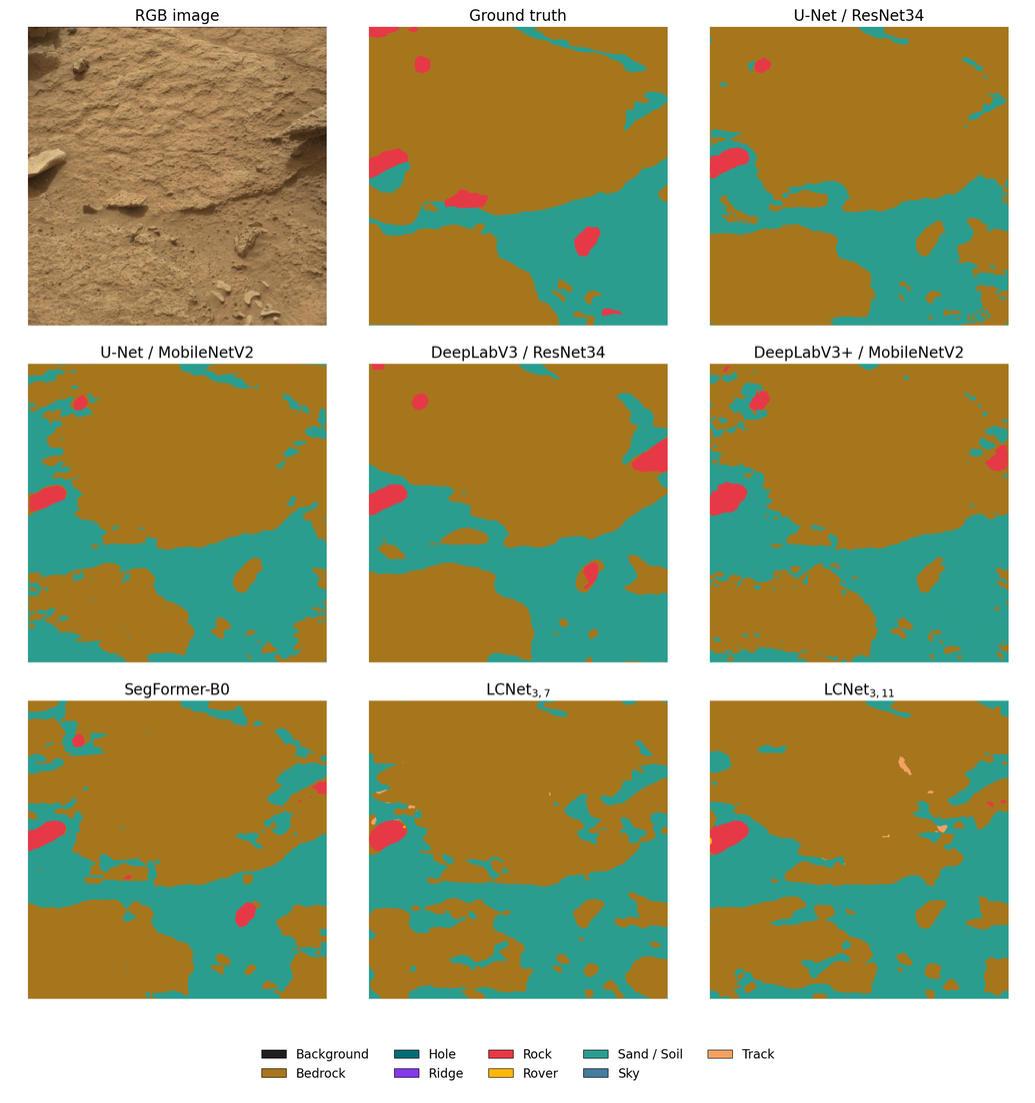
\includegraphics[width=\textwidth]{Images/s5mars_model_prediction_comparison.png}
    \caption{Qualitative comparison on an S5Mars test image, showing the RGB input, ground truth, and predictions of the seven evaluated configurations with a shared class colour mapping.}
    \label{fig:s5mars-model-prediction-comparison}
\end{figure}

\section{Quantization Results}
\label{sec:quantization-results}

Table~\ref{tab:s5mars-quantization-accuracy-efficiency} compares the previous results with the PTQ and QAT deployment variants described in Section~\ref{sec:optimization-quantization}. Accuracy was still evaluated on the S5Mars test split, whereas latency, energy per image, and peak GPU memory were measured through separate inference benchmarks with a batch size of one and an input resolution of \(512 \times 512\). LCNet was not included in this quantization campaign, given their already low parameter count and efficiency.

\begin{table}[ht!]
    \centering
    \small
    \setlength{\tabcolsep}{5pt}
    \begin{tabular}{@{}l r r r r r@{}}
        \toprule
        \textbf{Variant}                                    &
        \shortstack{\textbf{Test mIoU}\\\textbf{(\%)}}      &
        \shortstack{\textbf{\(\Delta\)mIoU}\\\textbf{(pp)}} &
        \shortstack{\textbf{Latency}\\\textbf{(ms)}}        &
        \shortstack{\textbf{Energy}\\\textbf{(mJ/image)}}   &
        \shortstack{\textbf{GPU peak}\\\textbf{(MiB)}}                                               \\
        \midrule
        \midrule

        \multicolumn{6}{@{}l}{\textit{U-Net (ResNet34)}}                                             \\
        FP32                                                & 64.55 & --    & 16.30 & 1213.08 & 1128 \\
        FP16                                                & 64.55 & 0.00  & 9.19  & 659.76  & 872  \\
        PTQ INT8                                            & 64.51 & -0.04 & 5.82  & 304.10  & 888  \\
        QAT INT8                                            & 65.24 & +0.69 & 4.81  & 231.42  & 1106 \\
        \midrule

        \multicolumn{6}{@{}l}{\textit{U-Net (MobileNetV2)}}                                          \\
        FP32                                                & 64.57 & --    & 11.87 & 878.80  & 1364 \\
        FP16                                                & 64.61 & +0.04 & 8.16  & 523.07  & 1236 \\
        PTQ INT8                                            & 61.55 & -3.02 & 4.17  & 199.96  & 1168 \\
        QAT INT8                                            & 65.00 & +0.42 & 3.57  & 162.66  & 912  \\
        \midrule

        \multicolumn{6}{@{}l}{\textit{DeepLabV3 (ResNet34)}}                                         \\
        FP32                                                & 73.79 & --    & 56.27 & 3977.25 & 414  \\
        FP16                                                & 73.79 & 0.00  & 14.03 & 1016.14 & 284  \\
        PTQ INT8                                            & 73.55 & -0.23 & 7.19  & 455.34  & 856  \\
        QAT INT8                                            & 73.62 & -0.17 & 8.65  & 523.71  & 1130 \\
        \midrule

        \multicolumn{6}{@{}l}{\textit{DeepLabV3+ (MobileNetV2)}}                                     \\
        FP32                                                & 64.07 & --    & 8.84  & 653.72  & 706  \\
        FP16                                                & 64.07 & 0.00  & 6.03  & 377.88  & 706  \\
        PTQ INT8                                            & 59.14 & -4.93 & 4.02  & 159.19  & 628  \\
        QAT INT8                                            & 65.63 & +1.57 & 3.01  & 115.34  & 450  \\
        \midrule

        \multicolumn{6}{@{}l}{\textit{SegFormer-B0}}                                                 \\
        FP32                                                & 75.55 & --    & 11.88 & 835.72  & 1550 \\
        FP16                                                & 75.55 & 0.00  & 7.17  & 432.07  & 1294 \\
        PTQ INT8                                            & 75.60 & +0.05 & 5.92  & 327.99  & 1118 \\
        QAT INT8                                            & 76.93 & +1.38 & 5.66  & 291.76  & 1008 \\
        \bottomrule
    \end{tabular}

    \vspace{5mm}
    \caption{
        Accuracy and inference resource measurements for the selected
        configurations. Latency is the mean forward pass time
        with inputs already on the device, excluding preprocessing.
        Peak GPU memory includes the resident model or engine and
        buffers. FP32 and FP16 use ONNX Runtime CUDA, PTQ uses ONNX
        Runtime TensorRT with fallback, and QAT uses TensorRT directly.
        INT8 denotes selective mixed-precision execution, with
        Conv-only quantization for SegFormer-B0.
    }
    \label{tab:s5mars-quantization-accuracy-efficiency}
\end{table}

FP16 conversion left test accuracy essentially unchanged across all five models, with the largest absolute mIoU difference remaining below 0.04\%. Across the five FP32-FP16 comparisons, the reported energy reduction ranged from 40.5\% to 74.5\%. PTQ introduced larger, model-dependent accuracy changes. U-Net with ResNet34 lost 0.04\%, SegFormer-B0 gained 0.05\%, and DeepLabV3 with ResNet34 lost 0.23\%. The two MobileNetV2 configurations were more sensitive in these experiments: U-Net lost 3.02\% and DeepLabV3+ lost 4.93\%, despite their lower latency and energy consumption.

The selected QAT configurations exceeded the corresponding FP32 test mIoU for four of the five models. SegFormer-B0 reached 76.93\%, an increase of 1.38\%, while DeepLabV3+ with MobileNetV2 reached 65.63\%, an increase of 1.57\%. DeepLabV3 with ResNet34 remained slightly below its FP32 counterpart, with a decrease of 0.17 points. These results describe the complete QAT optimization procedure, which included supervised fine-tuning and teacher distillation.

Figure~\ref{fig:s5mars-quantization-miou-energy} shows test mIoU versus measured GPU energy per image for the 20 examined configurations. Among these recorded points, QAT DeepLabV3+ and QAT SegFormer-B0 define the observed accuracy-energy frontier: neither has an alternative with both no greater energy consumption and no lower mIoU. DeepLabV3+ required the least measured energy, 115.34~mJ per image, whereas SegFormer-B0 provided the highest test mIoU at 291.76~mJ per image. Their comparison illustrates the remaining choice between a lower inference energy budget and more accurate segmentation, rather than identifying one configuration as preferable for every deployment requirement.

\begin{figure}[ht!]
    \centering
    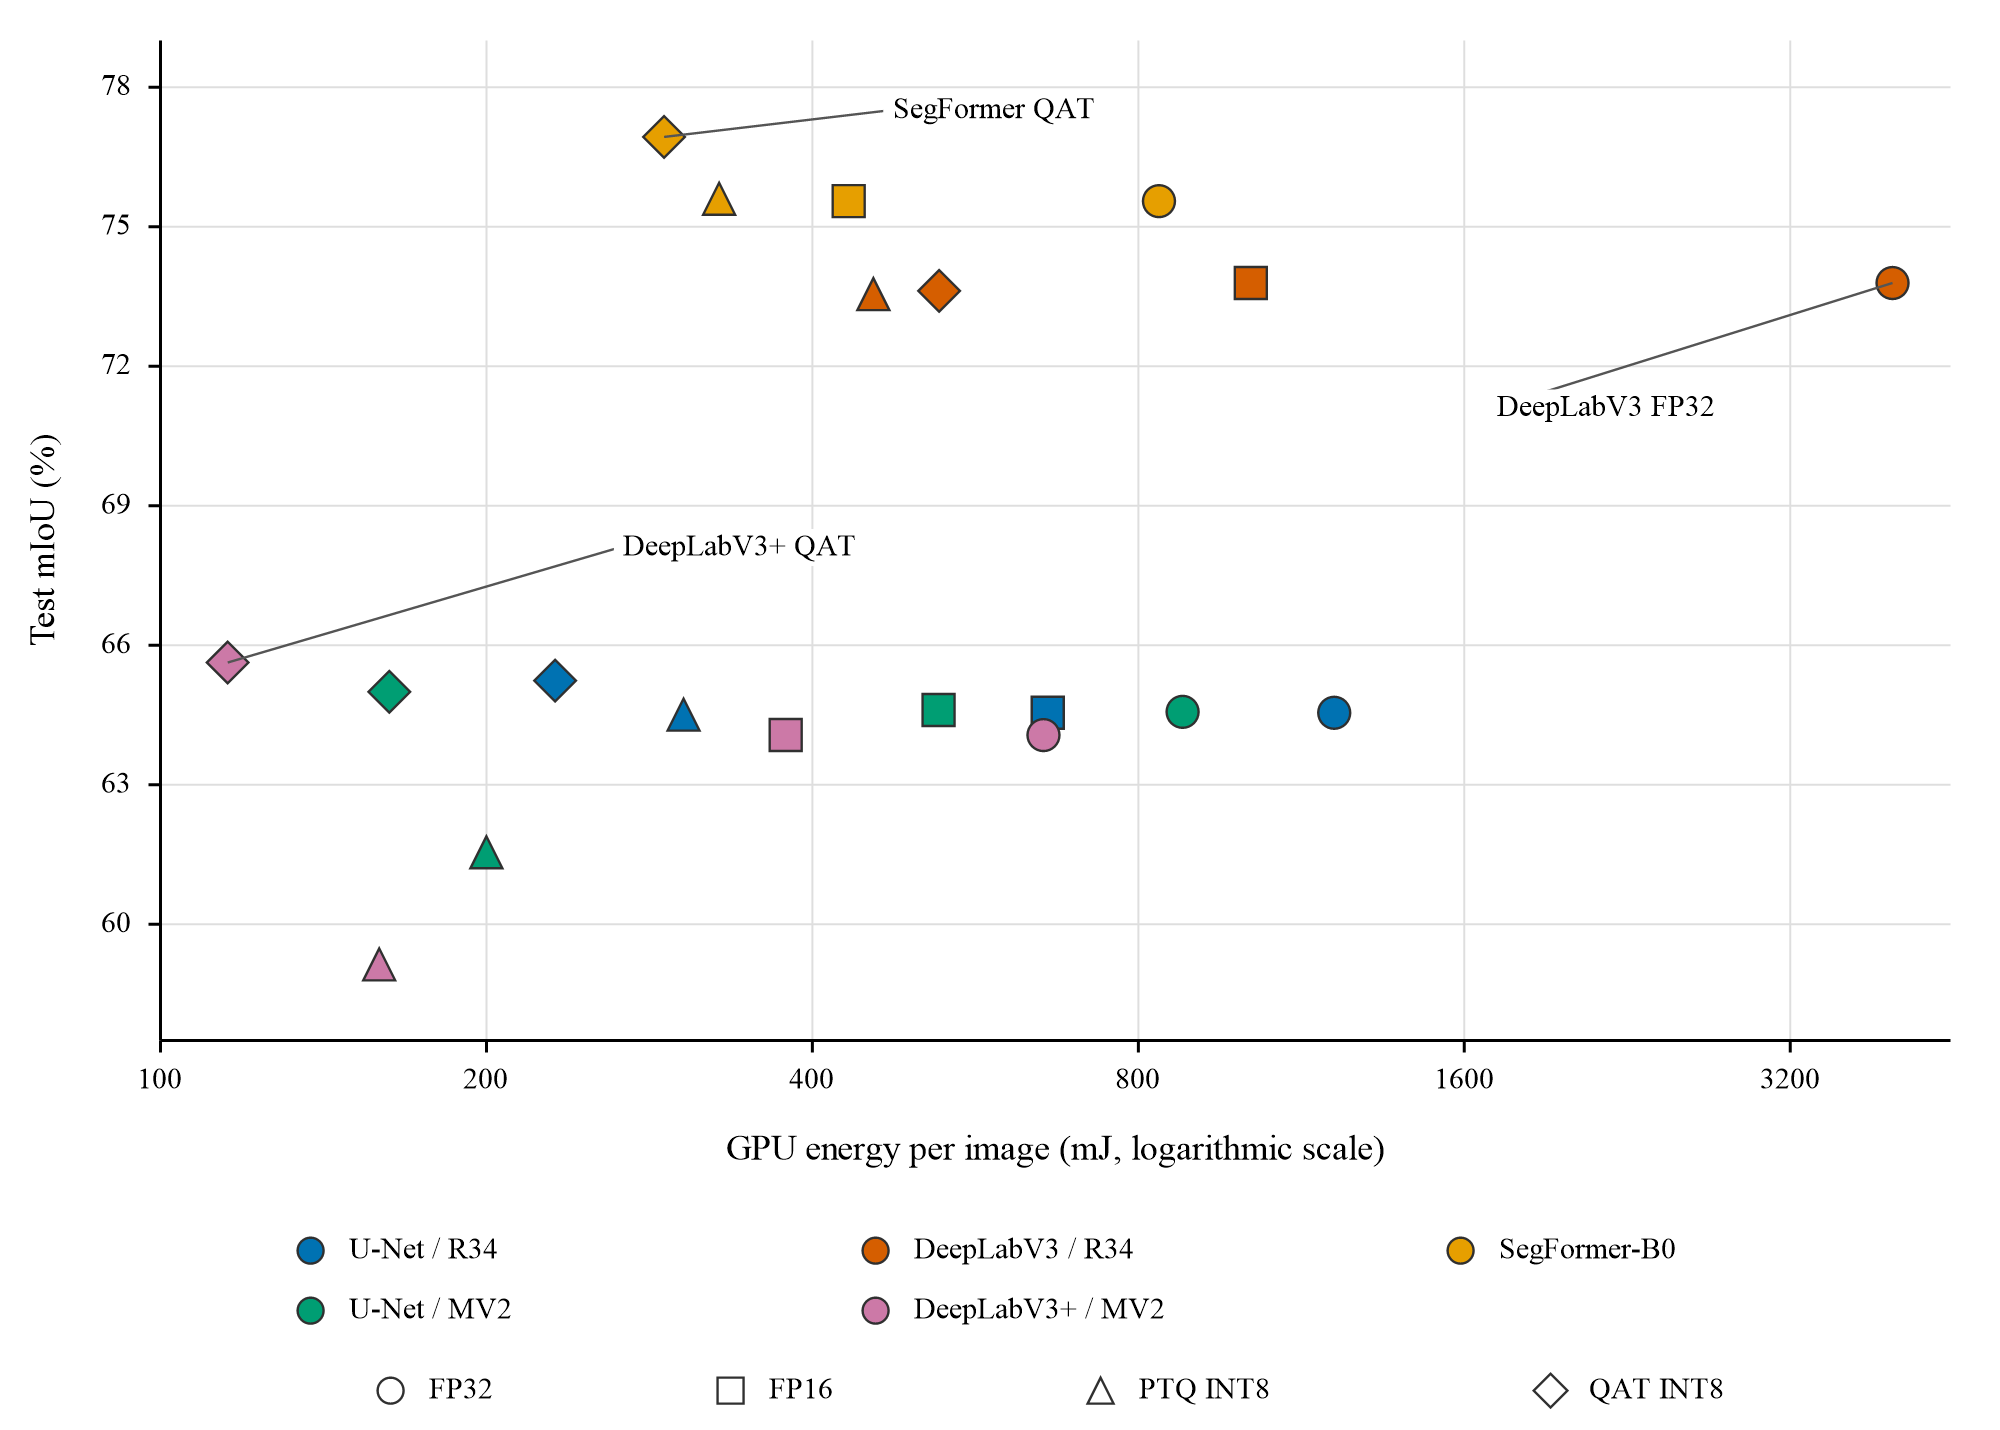
\includegraphics[width=\textwidth]{Images/quantization_miou_energy.png}
    \caption{Test mIoU versus GPU energy per image for the various configurations, with energy shown on a logarithmic scale. Colours identify the model and marker shapes identify the precision or quantization strategy. Lower energy and higher mIoU are preferable. The two QAT annotations identify the best configurations among the reported measurements, while the DeepLabV3 FP32 annotation highlights its higher energy consumption.}
    \label{fig:s5mars-quantization-miou-energy}
\end{figure}

Resource improvements were not uniform across all measurements. For U-Net with ResNet34, the QAT engine reduced latency and energy but used 1106~MiB of peak GPU memory, compared with 872~MiB for FP16. DeepLabV3 QAT also used more energy than its PTQ counterpart, 523.71 versus 455.34~mJ per image, despite its slightly higher accuracy. Since the execution backends and floating point fallback differ, these comparisons concern complete deployment configurations rather than isolating the effect of bit width. Furthermore, energy was estimated over a sustained GPU inference loop, includes device idle consumption, and excludes CPU energy. It is not an end-to-end system measurement or evidence of equivalent savings on rover flight hardware.

\section{Ablation Studies}
\label{sec:segmentation-ablation-studies}

The ablation studies investigate how the training strategy and quantization scope affect segmentation accuracy, providing an experimental basis for the configurations adopted in this study. The comparisons examine alternative loss formulations and class-weighting schemes, encoder initialization, data augmentation, and oversampling to assess whether these choices improve mIoU relative to their default settings. Quantization experiments were also conducted to test whether extending INT8 conversion to additional model components preserves segmentation accuracy. Because of time constraints, some experiments were conducted on a subset of the segmentation models evaluated in this study.

\subsection{Loss Function and Class Weighting}

% Evidence: original experiment Timeline, entries of 4 and 9 July.
% https://docs.google.com/document/d/11GTkTgIXR0t03VsOXm4SB1oaA0jJPNN3a9KFPZnC5KQ/edit
The initial loss comparison examined the combination of Cross-Entropy and Generalized Dice Loss (GDL) over Cross-Entropy alone for both SegFormer-B0 and U-Net with ResNet34, using the checkpoint with the highest validation mIoU for each run. As shown in Table~\ref{tab:s5mars-exploratory-loss-ablation}, test mIoU increased from 69.2\% to 73.7\% for SegFormer-B0 and from 64.5\% to 70.1\% for U-Net with ResNet34. These trials motivated the use of the combined objective with \(\alpha = 0.5\), which gives equal coefficients to pixel-wise classification and region-overlap supervision. Standalone GDL was also tried during preliminary experimentation but was not stable, so no numerical result is reported for that configuration.

\begin{table}[ht!]
    \centering
    \small
    \setlength{\tabcolsep}{5pt}
    \begin{tabular}{@{}l c c@{}}
        \toprule
        \textbf{Model}   & \textbf{CE} & \textbf{CE + GDL} \\
        \midrule
        \midrule
        SegFormer-B0     & 69.2        & 73.7              \\
        U-Net / ResNet34 & 64.5        & 70.1              \\
        \bottomrule
    \end{tabular}
    \vspace{5mm}
    \caption{Approximate test mIoU (\%). CE + GDL used inverse-square Dice weights.}
    \label{tab:s5mars-exploratory-loss-ablation}
\end{table}

Class weighting was tested to assess whether increasing the Dice contribution of classes occupying fewer pixels improved segmentation accuracy. Table~\ref{tab:s5mars-exploratory-dice-weighting} compares the three GDL weighting schemes for U-Net with ResNet34. Inverse-square weighting (\texttt{square}) achieved a test mIoU of 70.1\%, compared with 64.2\% for uniform weighting and 57.2\% for inverse-class-volume weighting (\texttt{simple}). These exploratory results motivated the use of inverse-square weighting in subsequent experiments. The interaction between this weighting scheme and oversampling is examined separately below.

\begin{table}[ht!]
    \centering
    \small
    \setlength{\tabcolsep}{5pt}
    \begin{tabular}{@{}l c c c@{}}
        \toprule
        \textbf{Model}   & \textbf{Inverse square} & \textbf{Inverse volume} & \textbf{Uniform} \\
        \midrule
        \midrule
        U-Net / ResNet34 & 70.1                    & 57.2                    & 64.2             \\
        \bottomrule
    \end{tabular}
    \vspace{5mm}
    \caption{Approximate test mIoU (\%) for U-Net with ResNet34 using CE + GDL and the three Dice-weighting schemes.}
    \label{tab:s5mars-exploratory-dice-weighting}
\end{table}

\subsection{Effect of Pretraining}

The initialization experiment assessed whether ImageNet-pretrained encoder weights provided a useful starting point for learning Martian scene segmentation. U-Net with ResNet34 trained from random initialization reached a test mIoU of 51.6\%, much below the pretrained U-Net results reported above. This observation is consistent with a benefit from pretrained initialization for the tested model and supports keeping it in subsequent experiments.

\subsection{Effect of Data Augmentation}

% Evidence: SegFormer reference and augmentation history.json/test_metrics.json.
% Reference test: Drive 1V8TqPDClr6jI39Jp7jNX3giIZM3HcoQr.
% Augmented test: Drive 1EVKdHS397eHql34tAjqcVnvNG2pIwurP.
The augmentation experiment tested whether adding transformed versions of the training images could help SegFormer-B0 perform better on unseen S5Mars images. The tested policy combined horizontal and vertical flips with random right-angle rotations. With standard sampling and inverse-square Dice weights, enabling this policy reduced validation mIoU from 80.28\% to 73.99\%, as shown in Table~\ref{tab:s5mars-segformer-training-ablation}. Test mIoU also fell from 75.55\% to 66.86\%. The extra geometric variation therefore did not improve accuracy in this experiment, therefore motivating keeping data augmentation disabled in the default configuration, while the test result shows the same pattern on unseen images.

\begin{table}[ht!]
    \centering
    \small
    \setlength{\tabcolsep}{5pt}
    \begin{tabular}{@{}l c c r r@{}}
        \toprule
        \textbf{Sampling}                              & \textbf{Dice weights} & \textbf{Augmentation} &
        \shortstack{\textbf{Val. mIoU}\\\textbf{(\%)}} &
        \shortstack{\textbf{Test mIoU}\\\textbf{(\%)}}                                                                 \\
        \midrule
        \midrule
        Standard                                       & \texttt{square}       & Disabled              & 80.28 & 75.55 \\
        Standard                                       & \texttt{square}       & Enabled               & 73.99 & 66.86 \\
        Oversampling                                   & \texttt{square}       & Disabled              & 70.64 & 71.02 \\
        Oversampling                                   & \texttt{uniform}      & Disabled              & 79.28 & 72.90 \\
        \bottomrule
    \end{tabular}
    \vspace{5mm}
    \caption{SegFormer-B0 training variants evaluated using the checkpoints with the highest validation mIoU in their respective training histories. All variants used the combined CE-GDL loss function. \texttt{square} denotes inverse-square class-volume weighting within GDL. Augmentation and oversampling were restricted to training, leaving validation and test samples unchanged.}
    \label{tab:s5mars-segformer-training-ablation}
\end{table}
% Evidence: oversampling test_metrics.json, square and uniform variants.
% Square: Drive 1s_l_TyB95OB8MKnpYZxyBpOtJ1FeOwLl.
% Uniform: Drive 1MDyDKpOWjn5CrlWKmub8_dgRWnfQ1qWH.
The oversampling experiment tested whether showing images containing rare classes more often during training could improve SegFormer-B0 accuracy on unseen S5Mars images. It also examined whether uniform Dice weights worked better than inverse-square weights when oversampling was enabled. As shown in Table~\ref{tab:s5mars-segformer-training-ablation}, oversampling with inverse-square weights produced lower validation and test mIoU than standard sampling: 70.64\% versus 80.28\% on validation and 71.02\% versus 75.55\% on test. Switching to uniform weights raised the oversampled run to 79.28\% on validation and 72.90\% on test, but both scores remained below the default. These results support keeping standard sampling with inverse-square Dice weights in the default configuration, with the validation and test scores showing the same trend. The benefit of uniform weights was observed within the oversampled runs, probably due to the work of square weights being done in part by oversampling.

%\subsection{Quantization Scope}
% TODO
% PTQ evidence: semantic_segmentation/docs/quantization/onnx_ptq_results.md,
% final SegFormer Conv+MatMul comparison (validation 200, test 800).
% QAT evidence: Conv-only Drive 1Kq-yIOds3hbGkVQPjJ8wi-uDNuhLpPyE;
% extended scope Drive 1ASZu4lePsdCcs28pVs4e_IkEoqJLd-Ge (no test result).
%The SegFormer experiments also examined how extending the INT8 scope affected segmentation accuracy. In PTQ, adding matrix multiplications to the Conv-only scope reduced test mIoU from 75.60\% to 75.12\%, as reported in Table~\ref{tab:s5mars-quantization-scope-ablation}. This deployment variant also moved convolutional biases into floating-point addition operations for TensorRT compatibility, so the comparison does not isolate the effect of quantizing matrix multiplications alone.

% \begin{table}[ht!]
%     \centering
%     \small
%     \setlength{\tabcolsep}{5pt}
%     \begin{tabular}{@{}l l r r@{}}
%         \toprule
%         \textbf{Method}                                & \textbf{INT8 scope}                                                       &
%         \shortstack{\textbf{Val. mIoU}\\\textbf{(\%)}} &
%         \shortstack{\textbf{Test mIoU}\\\textbf{(\%)}}                                                                                             \\
%         \midrule
%         \midrule
%         PTQ                                            & Convolutions only                                                         & 79.82 & 75.60 \\
%         PTQ                                            & Convolutions and matrix multiplications                                   & 79.53 & 75.12 \\
%         \midrule
%         QAT                                            & Convolutions only                                                         & 83.00 & 76.93 \\
%         QAT                                            & \shortstack[l]{Convolutions, encoder MLP\\and decoder linear projections} & 83.28 & --    \\
%         \bottomrule
%     \end{tabular}
%     \vspace{5mm}
%     \caption{SegFormer-B0 accuracy for different PTQ and QAT quantization scopes, measured on the deployed mixed-precision models rather than through fake-quantization evaluation. Unlisted operations remain floating point. The extended PTQ variant also changes convolutional bias handling. A dash denotes a test evaluation that was not performed.}
%     \label{tab:s5mars-quantization-scope-ablation}
% \end{table}

% The QAT extension instead quantized the linear layers in the encoder MLP blocks and decoder projections, while leaving attention computations in floating point. Validation mIoU increased from 83.00\% to 83.28\%. The extended configuration was not retained under the joint accuracy--efficiency selection criterion, and no held-out test result is available for it. Its validation gain therefore cannot be interpreted as an improvement in test performance over the Conv-only configuration.

\section{Cross-Mission Generalization on MarsSeg}
\label{sec:marsseg-cross-mission-generalization}

% Evidence: source test_metrics.json and cross_dataset_test JSONs from the
% six MarsSeg experiment folders, audited on 2026-10-05.
% https://drive.google.com/drive/folders/1t8bbQhbUIwbX6fOQZ45--8gfwyuhH7DS
The cross-mission experiment was designed to test whether a model trained on one rover mission could recognize the same terrain categories on another mission without additional training. This matters when labelled images from a new mission are scarce, and it also tests whether good results on the training mission translate into reliable generalization. MarsSeg MSL and MER were chosen because their Mars-Bench releases share the same terrain labels \cite{purohit2025marsbench}. S5Mars contains only Curiosity imagery and uses a different taxonomy, which would require remapping labels for a comparable cross-mission test.

SegFormer-B0, U-Net with ResNet34, and DeepLabV3+ with MobileNetV2 were each trained separately on MSL and MER. For each run, the checkpoint selected on the source validation split was tested on both the source mission and the other mission, with the same preprocessing and output labels. The cross-mission test used no target domain fine-tuning, giving a zero-shot measure of transfer. Models trained on the target mission provided a reference on the same test images, as reported in Table~\ref{tab:marsseg-cross-mission-accuracy}.

\begin{table}[ht!]
    \centering
    \small
    \setlength{\tabcolsep}{5pt}
    \begin{tabular}{@{}l r r r r@{}}
        \toprule
        \textbf{Model}                            &
        \multicolumn{2}{c}{\textbf{MSL training}} &
        \multicolumn{2}{c}{\textbf{MER training}}                                                                                 \\
        \cmidrule(lr){2-3}
        \cmidrule(l){4-5}
                                                  & \textbf{MSL test} & \textbf{MER test} & \textbf{MER test} & \textbf{MSL test} \\
        \midrule
        \midrule
        SegFormer-B0                              & 70.63             & \textbf{52.06}    & 66.75             & \textbf{48.11}    \\
        U-Net / ResNet34                          & \textbf{71.80}    & 27.43             & \textbf{67.76}    & 13.82             \\
        DeepLabV3+ / MobileNetV2                  & 68.98             & 38.27             & 65.10             & 12.86             \\
        \bottomrule
    \end{tabular}
    \vspace{5mm}
    \caption{Test mIoU (\%) for the MarsSeg cross-mission experiments. Each training mission identifies a separately trained model, evaluated on both test datasets. Evaluation on the other mission is zero-shot, without target-domain fine-tuning. Bold values indicate the highest recorded mIoU in each column.}
    \label{tab:marsseg-cross-mission-accuracy}
\end{table}

In-domain results were similar across the three configurations, with U-Net ranking first on both missions. Once the mission changed, SegFormer-B0 performed substantially better than both convolutional models in both directions. The CNNs struggled especially when trained on MER and tested on MSL, while SegFormer showed a more balanced transfer across the two missions. This answers the main question of the experiment, showing that high in-domain accuracy alone did not ensure good generalization, as even SegFormer lost accuracy compared with its target-trained references.

The smaller MER training set may partly explain why transfer from MER to MSL was harder for the convolutional models. With fewer examples, models may learn features that are too specific to the source images. Acquisition also differs: MSL provides RGB Mastcam images, whereas MER provides grayscale Navcam/Pancam images, and the images differ in their original dimensions \cite{purohit2025marsbench}. Such differences may make learned colour or texture patterns less useful on the other mission.

SegFormer's stronger transfer is consistent with its ability to combine local detail with larger scene context \cite{xie2021segformer}, together with its ADE20K segmentation pretraining. This initialization already provides features learned for pixel-level scene understanding, whereas the CNN encoders started from ImageNet classification weights, as described in Section~\ref{sec:segmentation-architectures}. Both factors may help when mission-specific training data are limited or image appearance changes. The results therefore support the evaluated Transformer configuration for cross-mission generalization.
